%!TEX root = ../thesis.tex

\subsection{Additive Noise Modelの識別可能条件}

本節では、連続変数データを扱うDAGモデルとして、
広く用いられているAdditive Noise Model(ANM)
\cite{Shimizu2006-yu}
\cite{Hoyer2008-oo}
\cite{Peters2013-eb}
\cite{Peters2014-ro}
\cite{Park2020-ey}
とその識別可能性について概説する。

ANMは、観測変数の同時分布が、
以下の構造方程式と誤差から生成されるDAGモデルである。

\begin{equation}
  X_j = f_j(X_{Pa(j)}) + e_j , \quad e_j \sim (0, \sigma_j^2)
  \label{def:ANM}
\end{equation}

ここで、$(f_j)_{j\in V}$は任意の関数であり、
$(e_j)_{j\in V}$は平均ゼロでそれぞれ異なる分散$(\sigma_j^2)_{j\in V}$に従う
互いに独立な確率変数である。

また、ANMの特殊形として、$(f_j)_{j\in V}$が全て線形な関数で記述されるモデルを、
線形構造方程式モデル(SEM)という。
つまり、観測変数の同時分布が以下の線形方程式で定義されるDAGモデルである。

\begin{equation}
  X_j = \theta_j + \sum_{k \in Pa(j)} \theta_{jk} X_k + e_j, \quad e_j \sim (0, \sigma_j^2)
\end{equation}

ここで、それぞれの係数$\theta_{jk}$は、DAG $G$における頂点$k$から頂点$j$の
直接的な因果効果の大きさを表す。
つまり、頂点$k$が頂点$k$の親であるときは$\theta_{jk} \neq 0$であり、
それ以外のときは$\theta_{jk}=0$である。

これらのDAGモデルは、関数形や誤差変数の分布についていくつかの制約を課すと、
識別可能であることが証明されている。
代表的な識別可能条件について以下に簡単にまとめる。

\begin{itemize}
  \item
  全ての関数$(f_j)_{j \in V}$が非線形である非線形ANM\cite{Hoyer2008-oo}

  \item
  全ての関数$(f_j)_{j \in V}$が線形であり、
  観測変数$(X_j)_{j \in V}$または誤差変数$(e_j)_{j\in V}$のいずれかの確率分布が、
  非ガウス分布に従う線形非ガウス非巡回モデル(LiNGAM)\cite{Shimizu2006-yu}

  \item
  全ての関数$(f_j)_{j \in V}$が線形であり、
  誤差変数$e_j$の分散が全て等しい、または全て既知である線形ANM\cite{Peters2013-eb}
\end{itemize}

このように関数形や誤差分布に関する仮定を置くことで、様々な識別可能なANMが提案されてきた。
一方で、全ての関数形が非線形であることや、誤差分布が非ガウス分布に従うこと、誤差分布の分散が全て等しいこと
などの仮定はあまり現実的でないといった批判もある。
そこで、誤差変数の分散の大きさだけでなく、誤差変数に対する親変数の影響の大きさも加味することで、
関数形や誤差変数の分布の制約を受けない以下のような識別可能条件が提案されている\cite{Park2020-ey}。

\begin{theo}[ANMの識別可能条件\cite{Park2020-ey}]
  同時確率$f(X)$がDAG $G$のANM(\ref{def:ANM})から生成されているとする。
  このとき、以下の2つの条件のいずれかが満たされているならば、
  DAG $G$は一意に識別可能である。
  ここでDAG $G$における因果順序を$\pi$で表す。

  任意の頂点$j = \pi_m \in V, k \in De(j), l \in An(j)$に関して、
  \begin{align*}
    (\text{A}) \quad &\sigma_j^2 < \sigma_k^2 + E(\mathit{Var}(E(X_k | X_{Pa(k)}) | X_{\pi_1}, \dots, X_{\pi_{m-1}})) \\
    (\text{B}) \quad &\sigma_j^2 > \sigma_l^2 - E(\mathit{Var}(E(X_l | X_{\pi_1}, \dots, X_{\pi_m} \backslash X_l) | X_{Pa(l)}))
  \end{align*}
\end{theo}

条件(A)は、頂点$j$の条件付き分散が、
非子孫$Nd(j)$で条件づけたときの$De(j)$の条件付き分散より小さいときに、
ANMは識別可能であることを表現している。
また、条件(B)は、頂点$j$の条件付き分散が、
祖先$An(j)$の親と子孫の和集合で条件づけたときの$An(j)$の条件付き分散より大きいときに、
ANMは識別可能であることを表現している。

ここでは条件(A)について直感的な理解を得るために、
図\ref{fig:ex_bivariate_SEM}のDAGで表される
2変数の正規線形構造方程式モデルを用いて、その識別可能性を証明する。

\begin{itemize}
  \item
  $G_1 \colon X_1 = e_1,
   \quad X_2 = \theta_1 X_1 + e_2$

  \item
  $G_2 \colon X_1 = \theta_2 X_2 + e_1,
   \quad X_2 = e_2$

  \item
  ただし、全ての$j \in \{ 1,2 \}$について、$e_j \sim N(0, \sigma_j^2)$である。
\end{itemize}

\begin{figure}[h]
  \centering
  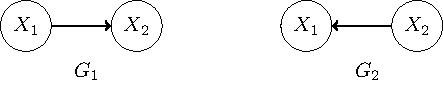
\includegraphics{./picture/bivariate_SEM.pdf}
  \caption{2変数の正規線形構造方程式モデル}
  \label{fig:ex_bivariate_SEM}
\end{figure}

$G_1$において、もし誤差変数の分散について条件(A)
$\sigma_1^2 < \sigma_2^2 + \beta_1^2 \sigma_1^2$が成立しているならば、
全分散の公式より$X_1$と$X_2$の分散について以下の関係が導かれる。

\begin{align*}
  \mathit{Var}(X_2) &= E(\mathit{Var}(X_2|X_1)) + \mathit{Var}(E(X_2|X_1)) \\
                    &= \sigma_2^2 + \beta_1^2 \sigma_1^2 \\
                    &> \sigma_1^2 \\
                    &= \mathit{Var}(X_1)
\end{align*}

この関係について直感的に述べると、
$X_1$における確率変動は$e_1$のみによって起こるが、
$X_2$における確率変動は$X_1$と$e_2$によって起こるため、
$X_2$の不確実性(分散)のほうが$X_1$の不確実性より大きくなると理解することができる。
よって、条件(A) $\sigma_1^2 < \sigma_2^2 + \beta_1^2 \sigma_1^2$が成立しているならば、
$G_1$における真の因果順序が$\pi = (1,2)$という順であることを観測変数より特定することができる。
